\documentclass[main.tex]{subfiles}
\begin{document}


\chapter{Concept} \label{chap:Concept}


\begin{figure}[H]
    \centering
    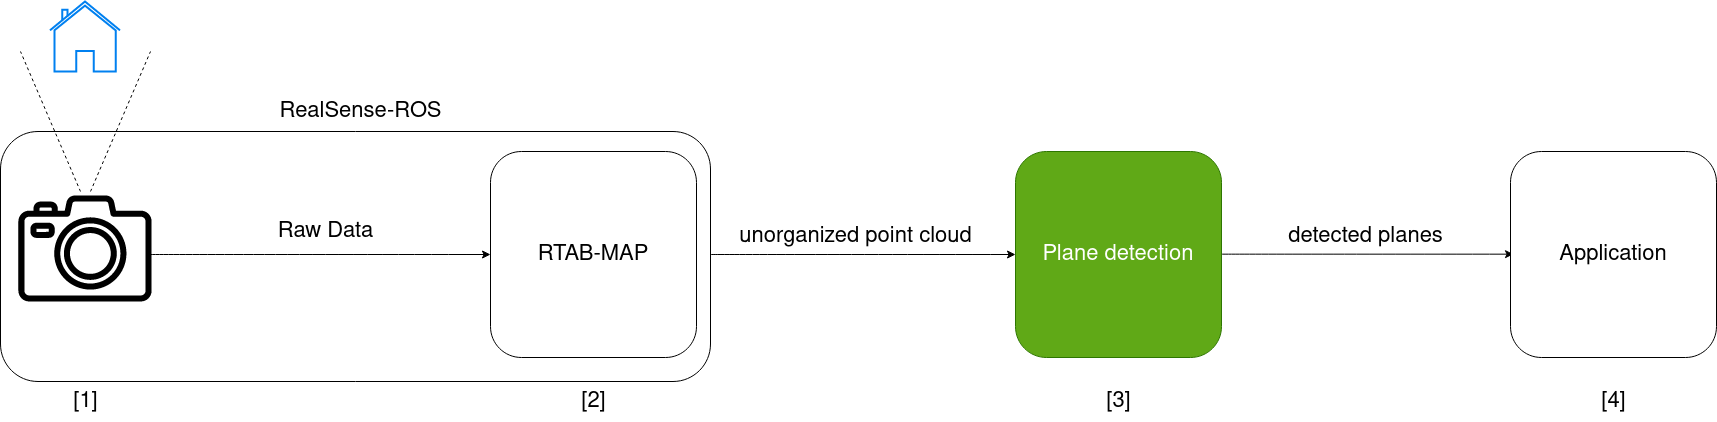
\includegraphics[width=15 cm]{images/concept_specific.png}
    \caption[AR/VR System Overview]{The procedure of the plane detection process. The specialized sensor records data ([1]), which is passed to
        a SLAM algorithm ([2]). After map assembly, a point cloud is handed to a plane detection algorithm ([3]).
        The detected planes are given to a use-case-specific application ([4]).}
    \label{fig:concept}
\end{figure}

Many AR and VR Systems integrate plane detection into their software, some use it only to calculate the ground floor while others use plane detection to
build a smaller model of the environment.
Figure~\ref{fig:concept} shows a generic block diagram of such a VR/AR system including plane detection.
In general, the environment is continuously recorded by a specialized sensor which is usually a camera([1]). A SLAM algorithm then integrates the new data into its already existing map([2]). The map, in form of a point cloud,
is subsequently passed to a plane detection algorithm([3]). The algorithm performs the necessary steps to detect all planes inside the current map and passes the planes to the application([4]).
The application would then further process those planes, e.g., by creating a live visualization of them or by assisting the movement of visually impaired people~\cite{Carranza_Estrella_Zaidi_Carranza_2021}.

To remove any noticeable delay in the application, the plane detection step has to run under a temporal restriction, henceforth referred to as \textit{real-time}.
We introduce a thorough definition of \textit{real-time} in Section~\ref{sec:realtime}.

When creating such an AR/VR system, the choice of plane detection algorithm is naturally of great importance. The problem is that most published algorithms are inherently incomparable.
Often different datasets or metrics are used, which precludes comparison by quantification.
Alternatively, algorithms are not comparable by internal functionality because many methods require other inputs, and the format of the planes differs accordingly.
All in all, selecting a single 'best' algorithm, solely based on the results presented in their respective work, is impossible.

To answer the question of which algorithm is best and whether it is real-time capable, we make a unified comparison of plane detection algorithms.
To perform this evaluation, we need the following:

\begin{enumerate}
    \item \label{enum:pda}Appropriate plane detection algorithms,
    \item \label{enum:ds} a useful dataset, \textit{and}
    \item \label{enum:rt} a definition of \textit{real-time}.
\end{enumerate}
The following sections are dedicated to these requirements.

\section{Selection of Plane Detection Algorithms}\label{sec:pdaselection}

Since most algorithms differ in certain aspects, it is not possible to compare them all uniformly.
Furthermore, not all algorithms are created out of the same motivation and, therefore, focus on different things.
Evaluating an algorithm in a scenario it has not been designed for would not yield meaningful results.
It is, therefore, necessary to first define objective criteria to superficially determine which algorithm seems to be relevant
for the context of this work.


\subsection{Criteria}
\label{subsec:criteria}
In the following paragraphs, we outline appropriate criteria for the objective assessment of plane detection algorithms.

\paragraph{Type of Input}\label{par:input}
The first criterion is the type of input expected by a plane detection algorithm.
Allowing vastly different input types is likely to render the evaluation more complicated, if not impossible because an equivalent transformation
between two input types is not always possible.

We detail the different types of input in Section~\ref{sec:dataformats}. To reiterate, the data representation of the recorded
environment falls into one of three categories:
\begin{itemize}
    \item \textit{unorganized} or \textit{unstructured point cloud} (UPC)
    \item \textit{organized} or \textit{structured point cloud} (OPC)
    \item image:
          \begin{itemize}
              \item Depth (DI)
              \item RGB (RGBI)
          \end{itemize}
\end{itemize}

OPC and UPC both describe point clouds in the cartesian coordinate system. The primary difference is that the 3D coordinates inside
an \textit{organized} point cloud are saved in a 2D grid, while the \textit{unorganized} point cloud resembles an unsorted 1D array.\\
Like OPC, depth images are a 2D grid of values. However, in contrast to the 3D coordinates of an OPC, the data points of depth images
are the distances to the sensor.



\paragraph{Detected Plane Format} \label{subsec:planeformat}
Which specific representation the detected planes take the form of is also essential.
If no uniform output type can be determined, consequently, no uniform metric for comparison can also be found.


Often the found planes are saved as a list of 3D points, henceforth referred to as inliers, which were assigned to a plane.
Another often used plane output format is the cartesian equation of a plane described by a normal vector $n$ and a vector $d$.

In methods that work on image data, found planes are often described by a segmentation mask (SM) or regions of pixels that belong together.

Finally, some methods use plane detection as a means to an end, e.g., for the reconstruction of a scene or the integration into
a SLAM architecture.

\paragraph{Hardware Requirements}
\label{par:hardware}
Another important aspect to consider is the hardware required by an algorithm.
Many applications in the field of robotics are limited in their processing power, often restricted to microcontrollers like
a Raspberry Pi\footnote{\href{https://www.raspberrypi.com/}{https://www.raspberrypi.com/}} or an Arduino\footnote{\href{https://www.arduino.cc/}{https://www.arduino.cc/}}.
Thus, most plane detection algorithms run on the \textit{CPU}, while some even implement some form of \textit{CPU} parallelism, e.g., 3D-KHT uses OpenMP\footnote{\href{https://www.openmp.org/}{https://www.openmp.org/}}
to speed up the octree construction~\cite[Section~4]{LimbergerOliveira2015HT3D}.
However, some methods are implemented either completely or partially on the \textit{GPU}.
For instance, \citeauthor{Hidalgo-Paniagua_Vega-Rodríguez_Pavón_Ferruz_2015}\cite{Hidalgo-Paniagua_Vega-Rodríguez_Pavón_Ferruz_2015} compare different
implementations of the RANSAC algorithm, whereas three versions are processed entirely on the \textit{CPU}, and the last one is offloaded
to the \textit{GPU} via CUDA\footnote{\href{https://developer.nvidia.com/cuda-toolkit}{https://developer.nvidia.com/cuda-toolkit}}.

To summarize, we differentiate between algorithms that run solely on the \textit{CPU} and algorithms that, additionally, employ the
machine's \textit{GPU}.

\paragraph{Availability}
Lastly, to use an algorithm, one has to be able to implement it. Some implementations are published alongside the corresponding paper.
Moreover, the availability of an implementation may be restricted by certain legalities.
While other publications are limited to the paper, the level of detail regarding the implementation details varies.

For further reference, we consider a plane detection algorithm to be \textit{available} if its implementation is successful, and
that the implementation does not involve a form of legal transaction.
\textbf{\textcolor{red}{die formulierung muss im grund aussagen, dass man seine seele nicht verkaufen muss um da ran zu kommen, dh
        im zweifel selber impl können, oder eine geg. nehmen. PEAC: formular ausfüllen wäre ne grauzone, aber daten sind ja kein geld oder? :')}}
\textbf{\textcolor{red}{dementsprechend sicher stellen dass die Y/N richtig sind}}

\subsection{Plane Detection Algorithms}
\label{subsec:pdaselect}
\textbf{\textcolor{red}{irgendwas zu "das ist logischerweise nicht alles, aber algorithmen die minuten brauchen haben wir gekonnt ignoriert"}}
A list of state-of-the-art algorithms is compiled through comprehensive research of the current literature on plane detection (see Table~\ref{tab:algos}).
The table shows the input type and the output format of all algorithms, as well as the required hardware, and the availability.
Note, that we consider all algorithms to be available, however, we are not aware of public implementations of OBRG and SCH-RG.
However, the respective publications outline their methods in high detail, thereby guiding a re-implementation.

\textbf{\textcolor{red}{PEAC?}}

The final output of \textit{PLaneNet, PlaneRecNet} and \textit{PlaneRCNN} is a piecewise-planar depth map of the input
image. Since modifying the architecture to return the segmentation masks and plane parameters would require minimal effort,
we adjusted the output types in the table accordingly. Similarly, \textit{RSPD} returns a set of planes parameterized by
its normal vector $n$, distance to origin $d$, and two additional extents. Modifying the output to return inliers requires
minimal effort as well.
\begin{table}[H]
    \centering
    \resizebox{\textwidth}{!}{%
        \begin{tabular}{c|c|c|c|c|c}
            \textbf{Plane Detection Algorithm}                               & \textbf{Input Data} & \textbf{Plane Format} & \textbf{Hardware} & \textbf{Available} & \textbf{Section}            \\ \hline
            \textbf{RSPD} \cite{Araújo_Oliveira_2020}                        & UPC                 & 3D-IN, $(n,d)$        & CPU               & Y                  & \ref{subsec:bg-rspd}        \\
            \textbf{OPS} \cite{Sun_Mordohai_2019}                            & UPC                 & 3D-IN                 & CPU               & Y                  & \ref{subsec:bg-ops}         \\
            \textbf{3DKHT} \cite{LimbergerOliveira2015HT3D}                  & UPC                 & 3D-IN                 & CPU               & Y                  & \ref{subsec:bg-3dkht}       \\
            \textbf{OBRG} \cite{Vo_Truong-Hong_Laefer_Bertolotto_2015}       & UPC                 & 3D-IN                 & CPU               & Y                  & \ref{subsec:bg-obrg}        \\
            \textbf{PEAC} \cite{Feng_Taguchi_Kamat_2014}                     & OPC                 & 2D-IN                 & CPU               & Y                  & \ref{subsec:bg-peac}        \\
            \textbf{CAPE} \cite{Proença_Gao_2018}                            & OPC                 & $(n, d)$              & CPU               & Y                  & \ref{subsec:bg-cape}        \\
            \textbf{SCH-RG} \cite{Mols_Li_Hanebeck_2020}                     & OPC                 & 2D-IN                 & GPU               & Y                  & \ref{subsec:bg-schrg}       \\
            \textbf{D-KHT}  \cite{Vera_Lucio_Fernandes_Velho_2018}           & DI                  & 2D-IN                 & CPU               & Y                  & \ref{subsec:bg-dkht}        \\
            \textbf{DDFF} \cite{Roychoudhury_Missura_Bennewitz_2021}         & DI                  & 2D-IN                 & CPU               & Y                  & \ref{subsec:bg-ddff}        \\
            \textbf{PlaneNet} \cite{Liu_Yang_Ceylan_Yumer_Furukawa_2018}     & RGBI                & 2D-IN, $(n, d)$       & GPU               & Y                  & \ref{subsec:bg-planenet}    \\
            \textbf{PlaneRecNet} \cite{Xie_Shu_Rambach_Pagani_Stricker_2022} & RGBI                & 2D-IN, $(n)$            & GPU               & Y                  & \ref{subsec:bg-planerecnet} \\
            \textbf{PlaneRCNN} \cite{Liu_Kim_Gu_Furukawa_Kautz_2019}         & RGBI                & 2D-IN, $(n, d)$       & GPU               & Y                  & \ref{subsec:bg-planercnn}   \\
        \end{tabular}
    }
    \caption{A list of Plane Detection Algorithms compiled by reviewing the current literature. The algorithms are clustered by their type of input.
        The rightmost column provides the placement within this work. We refer to Subsection~\ref{subsec:criteria} for details regarding the specific namings.}
    \label{tab:algos}
\end{table}

As mentioned above, we consider all presented algorithms available even if \textit{SCH-RG} and \textit{OBRG} do not seem to have an official implementation.
Therefore, while necessary, the \textit{availability} criterion does not constrain the selection of algorithms in this case.

As stated in Paragraph~\ref{par:hardware}, mobile robotics applications or AR/VR systems are often limited in their processing power.
Moreover, integrating an external GPU into the system poses an additional cost factor.
We exclude algorithms that require an external GPU, namely \textit{SCH-RG, PlaneNet, PlaneRecNet}, and \textit{PlaneRCNN}.

Addressing the criterion of \textit{input type}, we are only interested in performing plane detection in complete environments.
Each update published by RTAB-MAP is the union of new data and the current state of the recorded map. RTAB-MAP publishes this update
in form of an \textit{unorganized} point cloud (see Figure~\ref{fig:rtabmap}).
To perform plane detection with an algorithm that expects an \textit{organized} point cloud as input, the UPC has to be transformed into an OPC.
This transformation is not-trivial and involves the projection of 3D coordinates onto a sphere based on a set of sensor parameters.
An exemplary implementation thereof is included in the lidar toolbox of MATLAB\footnote{\href{https://de.mathworks.com/help/lidar/ug/unorgaized-to-organized-pointcloud-conversion.html}{https://de.mathworks.com/help/lidar/ug/unorgaized-to-organized-pointcloud-conversion.html}}.
However, this transformation neglects the global structure of the environment, as it returns a two-dimensional representation of the environment.
Therefore, we focus on \textit{unorganized} point clouds in this work and exclude \textit{PEAC, CAPE, SCH-RG, D-KHT, DDFF, PlaneNet, PlaneRecNet} and \textit{PlaneRCNN} from our evaluation.

The detected planes need to be in the same format because, even for the same plane, different representations could very well lead to different results.
Assume a plane in cartesian form ($n,d$) and a plane represented by its inliers (3D/2D). The calculated metrics may differ significantly because the plane in cartesian form is infinitely dense.
Conversely, the plane described by its inliers allows for holes and non-rectangular shapes, e.g., doorways or a round table, respectively.
Being able to represent planes of any shape is important for many applications. Moreover, only the 3D inliers $3D-IN$ conform to
the determined input type of $UPC$ (see Section~\ref{subsec:output}).
We thereby determine \textit{three-dimensional inliers} (3D-IN) as the preferred \textit{plane format} and exclude all methods which do not comply, namely \textit{CAPE, PlaneNet, PlaneRecNet}, and \textit{PlaneRCNN}.

Note, that 3D inliers are henceforth referred to solely as \textit{inliers}. 


Applying these restrictions, we end up with, and thus include, the following plane detection algorithms in our evaluation:

\begin{itemize}
    \item \textbf{RSPD}
    \item \textbf{OPS}
    \item \textbf{3D-KHT}
    \item \textbf{OBRG}
\end{itemize}

\paragraph{Temporal Subdivision in Phases}
\label{par:prepostalgos}
To enable a precise evaluation, we subdivide these plane detection algorithms into three phases:
The pre-processing phase, the plane detection phase, and the post-processing phase. Note, that
we use the terms "phase" and "step" interchangeably in this work. In the following, we outline
the pre-processing and post-processing steps taken by the selected algorithms. To avoid redundancy,
we refer the reader to the Subsections~\ref{subsec:bg-rspd}-\ref{subsec:bg-obrg} for a detailed explanation of each
algorithm.

The pre-and post-processing steps are summarized in Table~\ref{tab:pre-post}.
RSPD, 3D-KHT, and OBRG construct an octree (OC) during their pre-processing phase.
Additionally, RSPD and OBRG perform an initial estimation of normals (NE).
OPS estimates the normal vectors for a randomly chosen sample set of points of pre-determined size.

During post-processing, OPS merges smaller planes if they pass a coplanarity test and then re-estimates the normals of the
resulting plane. In the post-processing step, OBRG refines the borders of detected planes by inserting
previously unallocated regions. RSPD and 3D-KHT do not perform post-processing.


\begin{table}[H]
    \centering
    \begin{tabular}{c|cccc}
             & RSPD & OPS   & 3D-KHT & OBRG       \\ \hline
        Pre  & NE   & NE    & OC     & OC + NE    \\
        Post & /    & Merge & /      & Refinement
    \end{tabular}
    \caption{The Pre-processing and post-processing steps of the plane detection algorithms. "/" denotes the absence of
        a pre-/post-processing step.}
    \label{tab:pre-post}
\end{table}




\section{Datasets}
\label{sec:datasets}
As mentioned at the beginning of this chapter, we also need an appropriate dataset for the evaluation.
Through extensive research of current literature, we compiled a list of popular datasets (see Table~\ref{tab:datasets}).

\begin{table}[H]
    \centering
    \begin{tabular}{c|c|c|c|c|c}
        \textbf{Dataset}                                                                                                                                                                      & \textbf{Scene Format} & \textbf{Real} & \textbf{Indoor} & \textbf{GT} & \textbf{Section}         \\ \hline
        \textbf{2D-3D-S}      \cite{2017arXiv170201105A}                                                                                                                                      & UPC                   & Y             & Y               & objects     & \ref{subsec:bg-stanford} \\
        \textbf{Leica\tablefootnote{\href{https://shop.leica-geosystems.com/de/leica-blk/blk360/dataset-downloads}{https://shop.leica-geosystems.com/de/leica-blk/blk360/dataset-downloads}}} & UPC                   & Y             & N               & planes      & \ref{subsec:bg-Leica}    \\
        \textbf{Kinect}      \cite{Oehler_Stueckler_Welle_Schulz_Behnke_2011}                                                                                                                 & OPC                   & Y             & Y               & planes      & \ref{subsec:bg-Kinect}   \\
        \textbf{SYNPEB}      \cite{schaefer19icra}                                                                                                                                            & OPC                   & N             & /               & planes      & \ref{subsec:bg-SYNPEB}   \\
        \textbf{ARCO}        \cite{Hidalgo-Paniagua_Vega-Rodríguez_Pavón_Ferruz_2015}                                                                                                         & OPC                   & Y             & Y               & /           & \ref{subsec:bg-ARCO}     \\
        \textbf{SegComp}     \cite{article}                                                                                                                                                   & DI                    & N             & /               & planes      & \ref{subsec:bg-segcomp}  \\
        \textbf{NYU V2}      \cite{10.1007/978-3-642-33715-4_54}                                                                                                                              & DI                    & Y             & Y               & classes     & \ref{subsec:bg-NYU}      \\
        \textbf{ICL-NUIM}    \cite{handa:etal:ICRA2014}                                                                                                                                       & DI                    & Y             & Y               & trajectory  & \ref{subsec:bg-ICL}      \\
        \textbf{SUNRGB-D}         \cite{7298655}                                                                                                                                              & DI                    & Y             & Y               & objects     & \ref{subsec:bg-SUN}      \\
        \textbf{TUM}         \cite{sturm12iros}                                                                                                                                               & DI                    & Y             & Y               & trajectory  & \ref{subsec:bg-TUM}      \\ \hline
        \textbf{FIN (ours)}                                                                                                                                                                   & UPC                   & Y             & Y               & planes      & \ref{sec:finimpl}
    \end{tabular}
    \caption[Popular Datasets]{Plane detection Datasets. The \textit{GT}(Ground Truth) column specifies what the ground truth of each dataset represents.
        Note, that the synthetic datasets (e.g., SegComp and SYNPEB) represent neither indoor nor outdoor scenes, hence the "/" in
        the respective table entries. The datasets are clustered by their type of format. Moreover, the remaining order is arbitrary.
        The rightmost column provides the placement within this work.
        Note, that we include our dataset (FIN) in this table for completeness reasons.
    }
    \label{tab:datasets}
\end{table}
In Subsection~\ref{subsec:pdaselect}, we determine \textit{unorganized} point clouds as the type of input. Furthermore, we focus on plane detection in real environments in this work.
Because most datasets do not conform to these two requirements, only \textit{2D-3D-S} and \textit{Leica} remain.
Since we focus on plane detection in indoor environments, \textit{Leica} ceases to be an option.
Thus, we choose \textit{2D-3D-S} as the dataset for the evaluation.
% \textcolor{red}{\\beispiel bilder von 2d3ds ?}\newline

Nonetheless, we cannot use the provided ground truth of \textit{2D-3D-S} because it represents the segmented scene on the level of objects, rather than planes in the scene.
Consequently, we create an appropriate ground truth by manual segmentation of all planes in a given scene.
We outline the details thereof in Section~\ref{sec:gtseg}.

Lastly, \textit{2D-3D-S} does not inherit any temporal component, i.e., the \textit{unorganized} point clouds do not grow incrementally over time.
To the best of our knowledge, there exists no dataset that meets the above criteria and, additionally, provides a plane-focused ground truth.
Therefore, we record an incrementally growing dataset in the Faculty of Computer Science at Otto-von-Guericke University Magdeburg,
henceforth referred to as the \textit{FIN} dataset.



To perform a thorough comparison between the \textit{FIN} and \textit{2D-3D-S}, and, subsequently, between the static and the dynamic dataset, we record a scene for each of the following scene types:
\begin{itemize}
    \item office
    \item conference room
    \item auditorium
    \item hallway
\end{itemize}

We focus on these four scene types because they are the most common in a real indoor environment.
The recorded point clouds can be seen in Figure~\ref{fig:fin}.
Lastly, since this is a novel dataset and thus has no ground truth, we create a ground truth. The details thereof are explained in Section~\ref{sec:finimpl}.


\begin{figure}[H]
    \begin{subfigure}{0.5\textwidth}
        \centering
        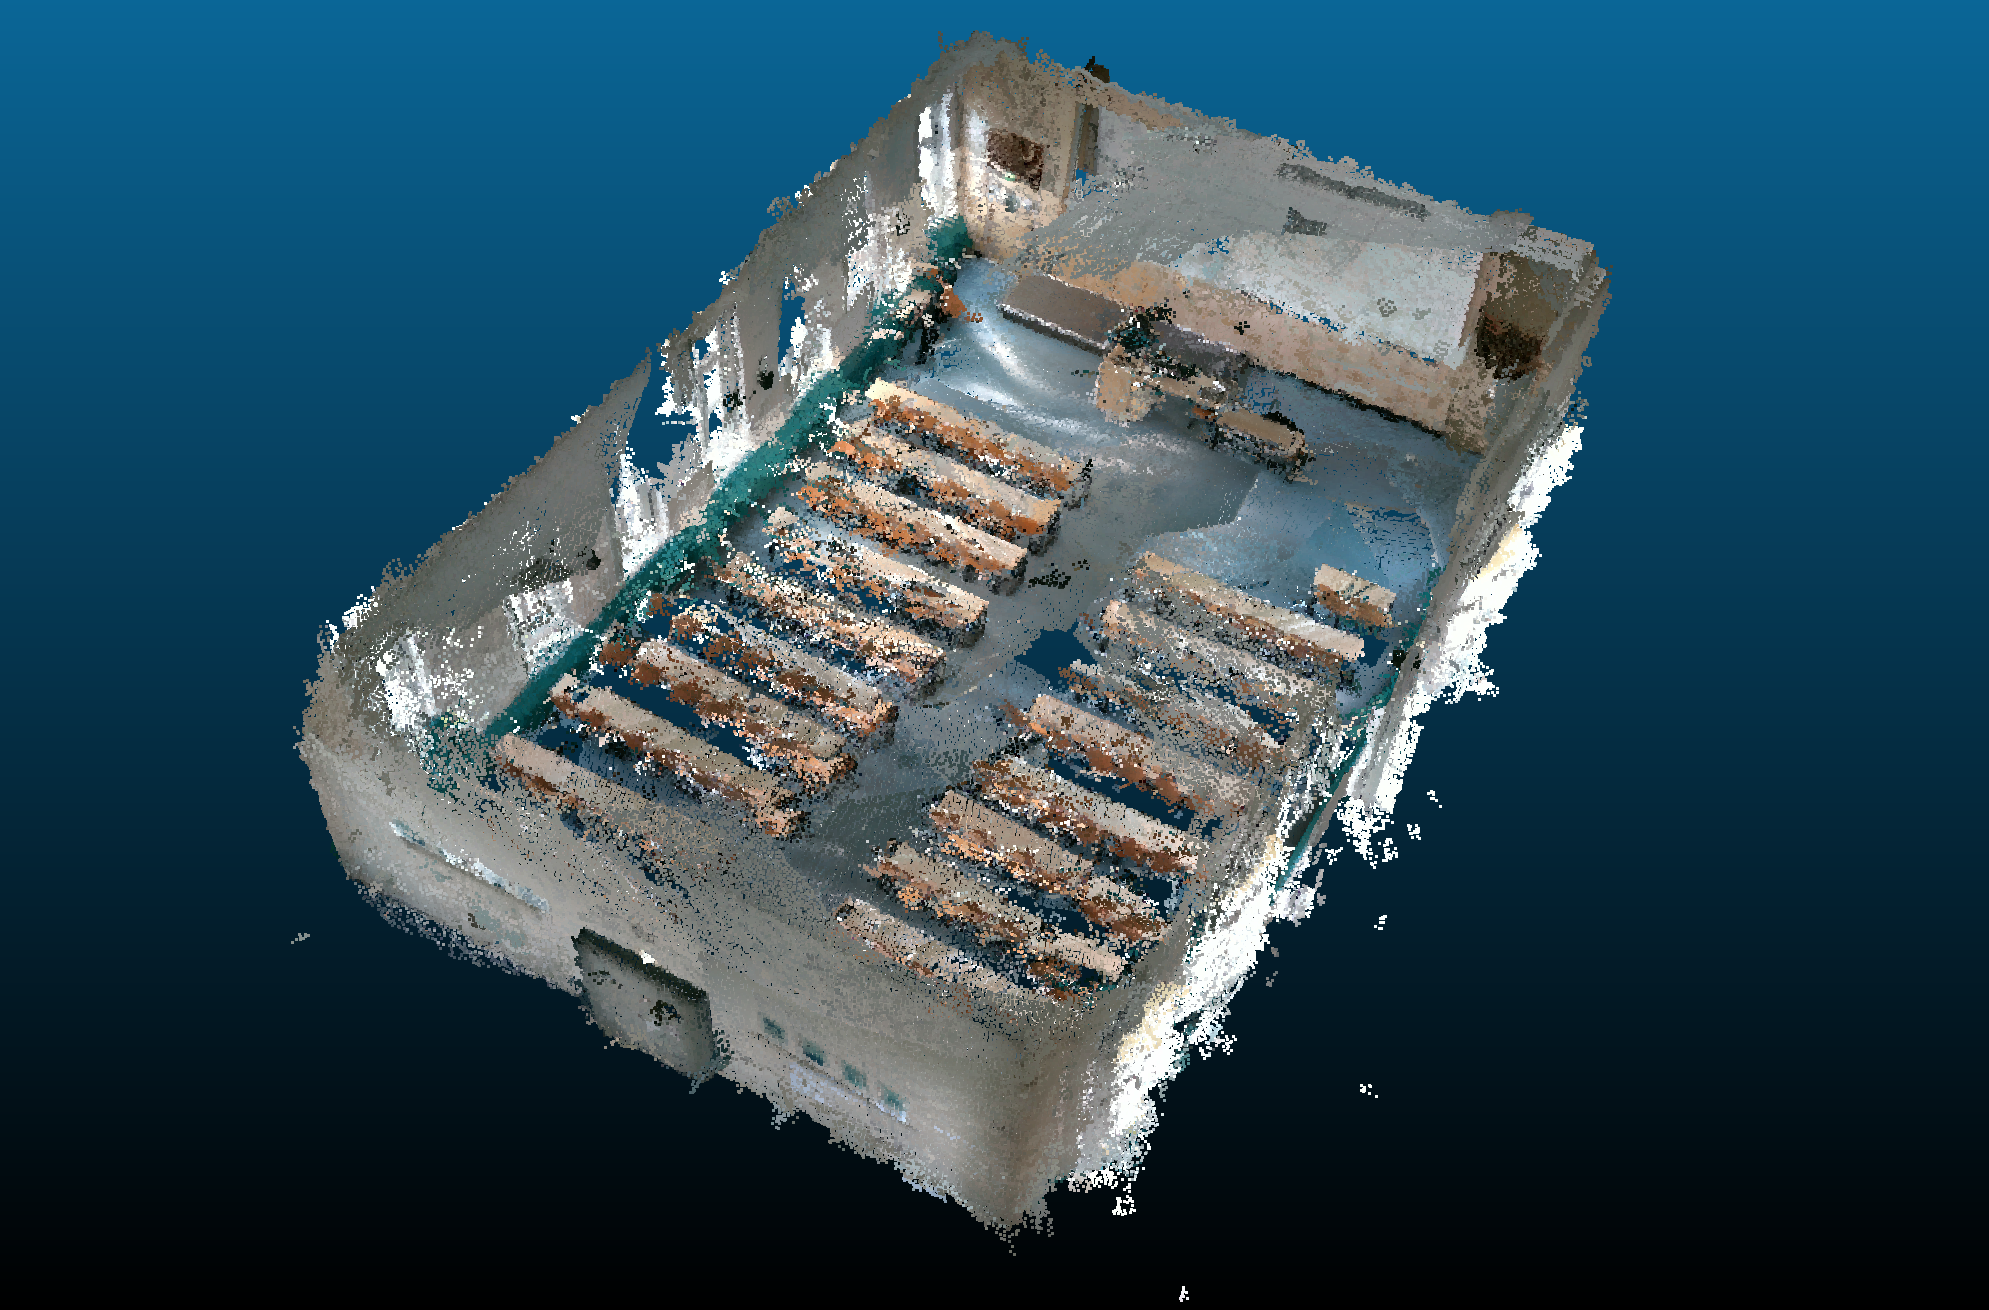
\includegraphics[width=.9\linewidth]{images/307.png}
        \caption[Dynamic Dataset - auditorium]{}
        \label{fig:fin307}
    \end{subfigure}
    \begin{subfigure}{0.5\textwidth}
        \centering
        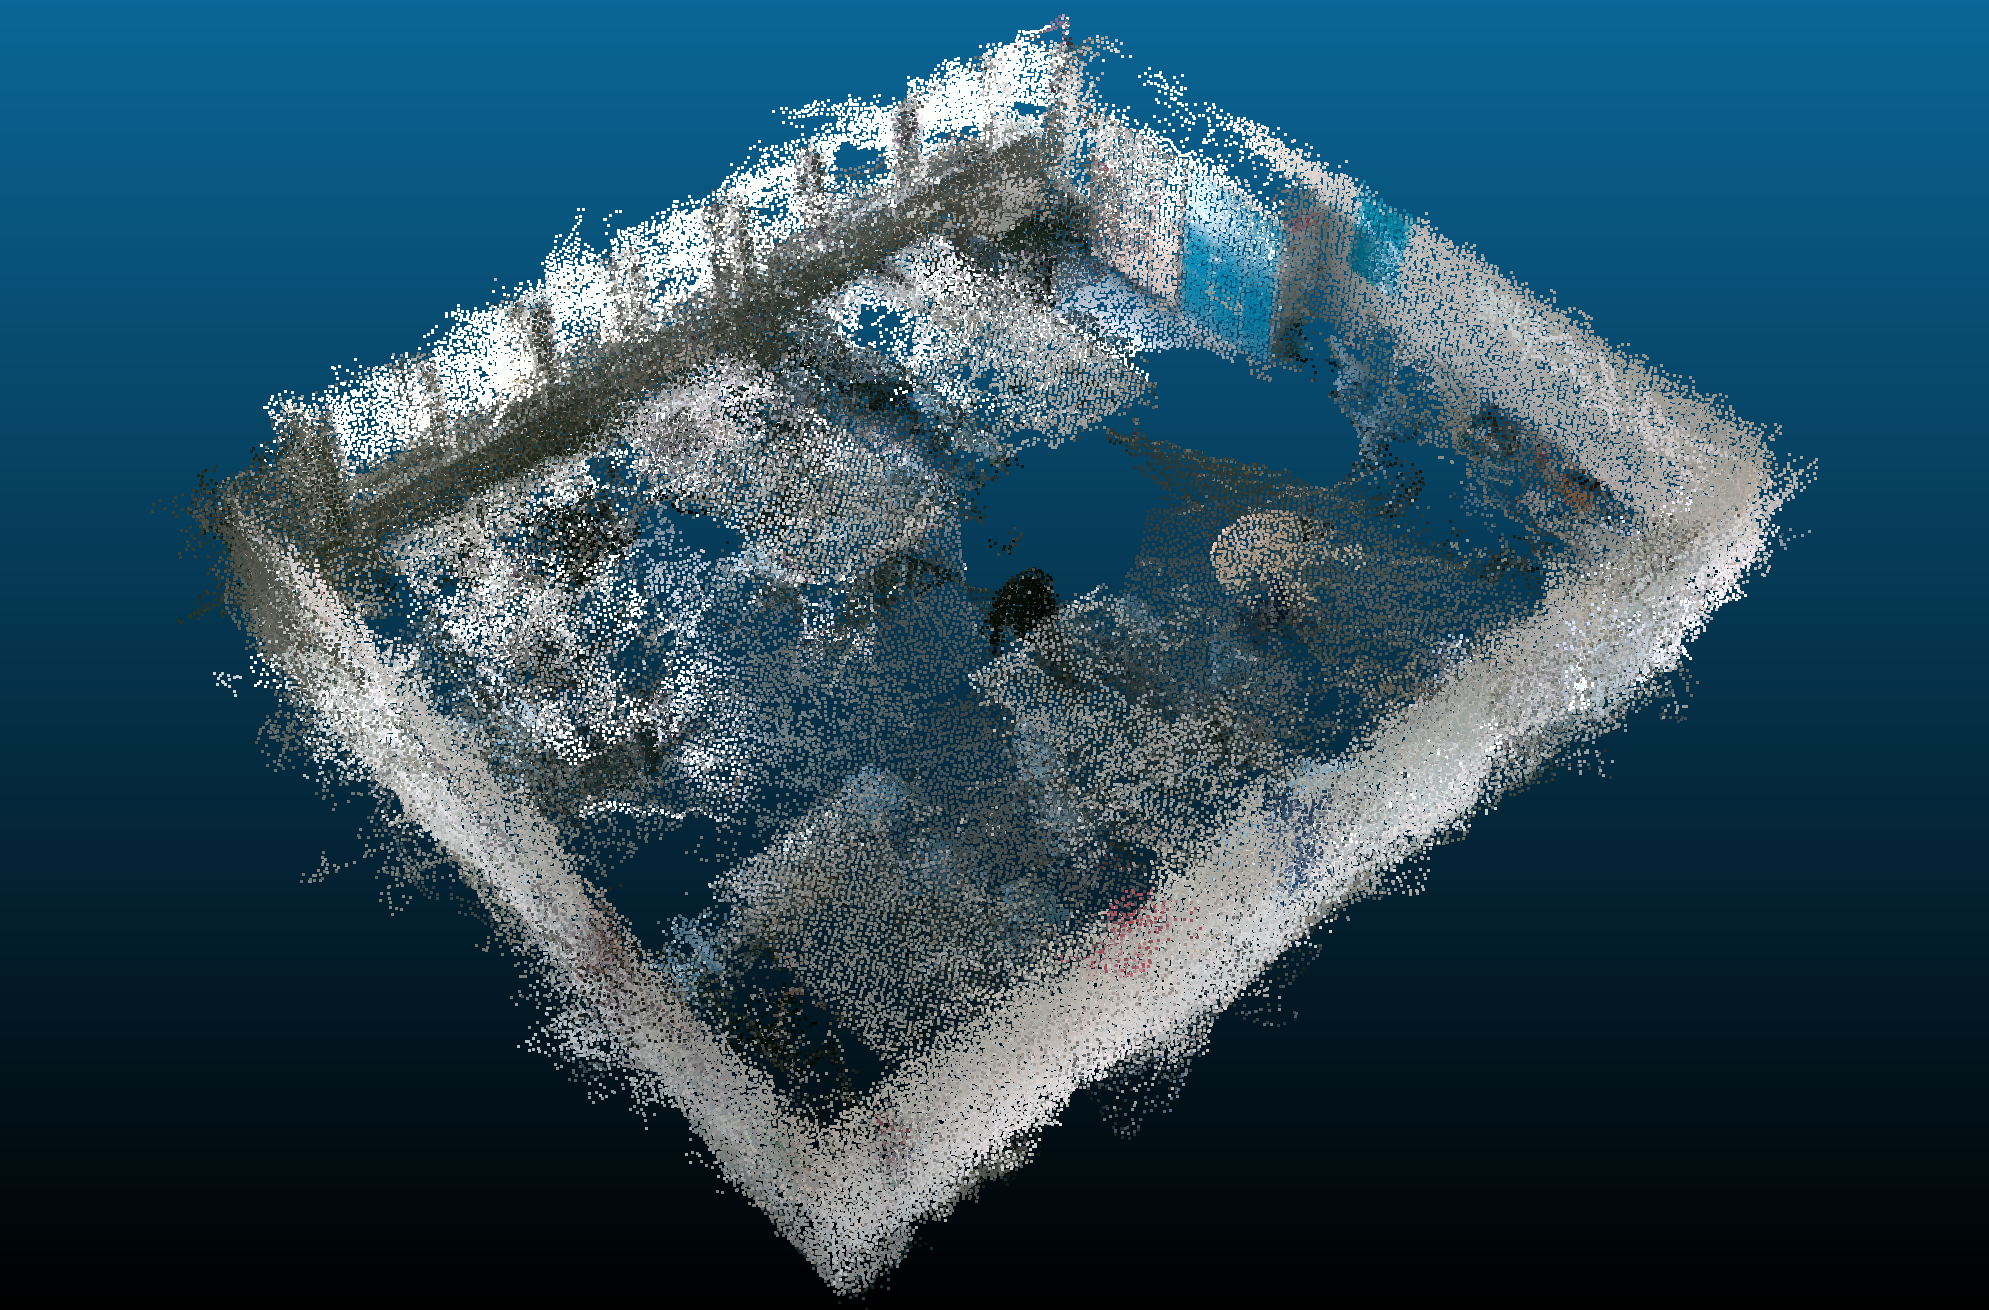
\includegraphics[width=.9\linewidth]{images/333.png}
        \caption[Dynamic Dataset - conference room]{}
        \label{fig:fin333}
    \end{subfigure}
    \begin{subfigure}{0.5\textwidth}
        \centering
        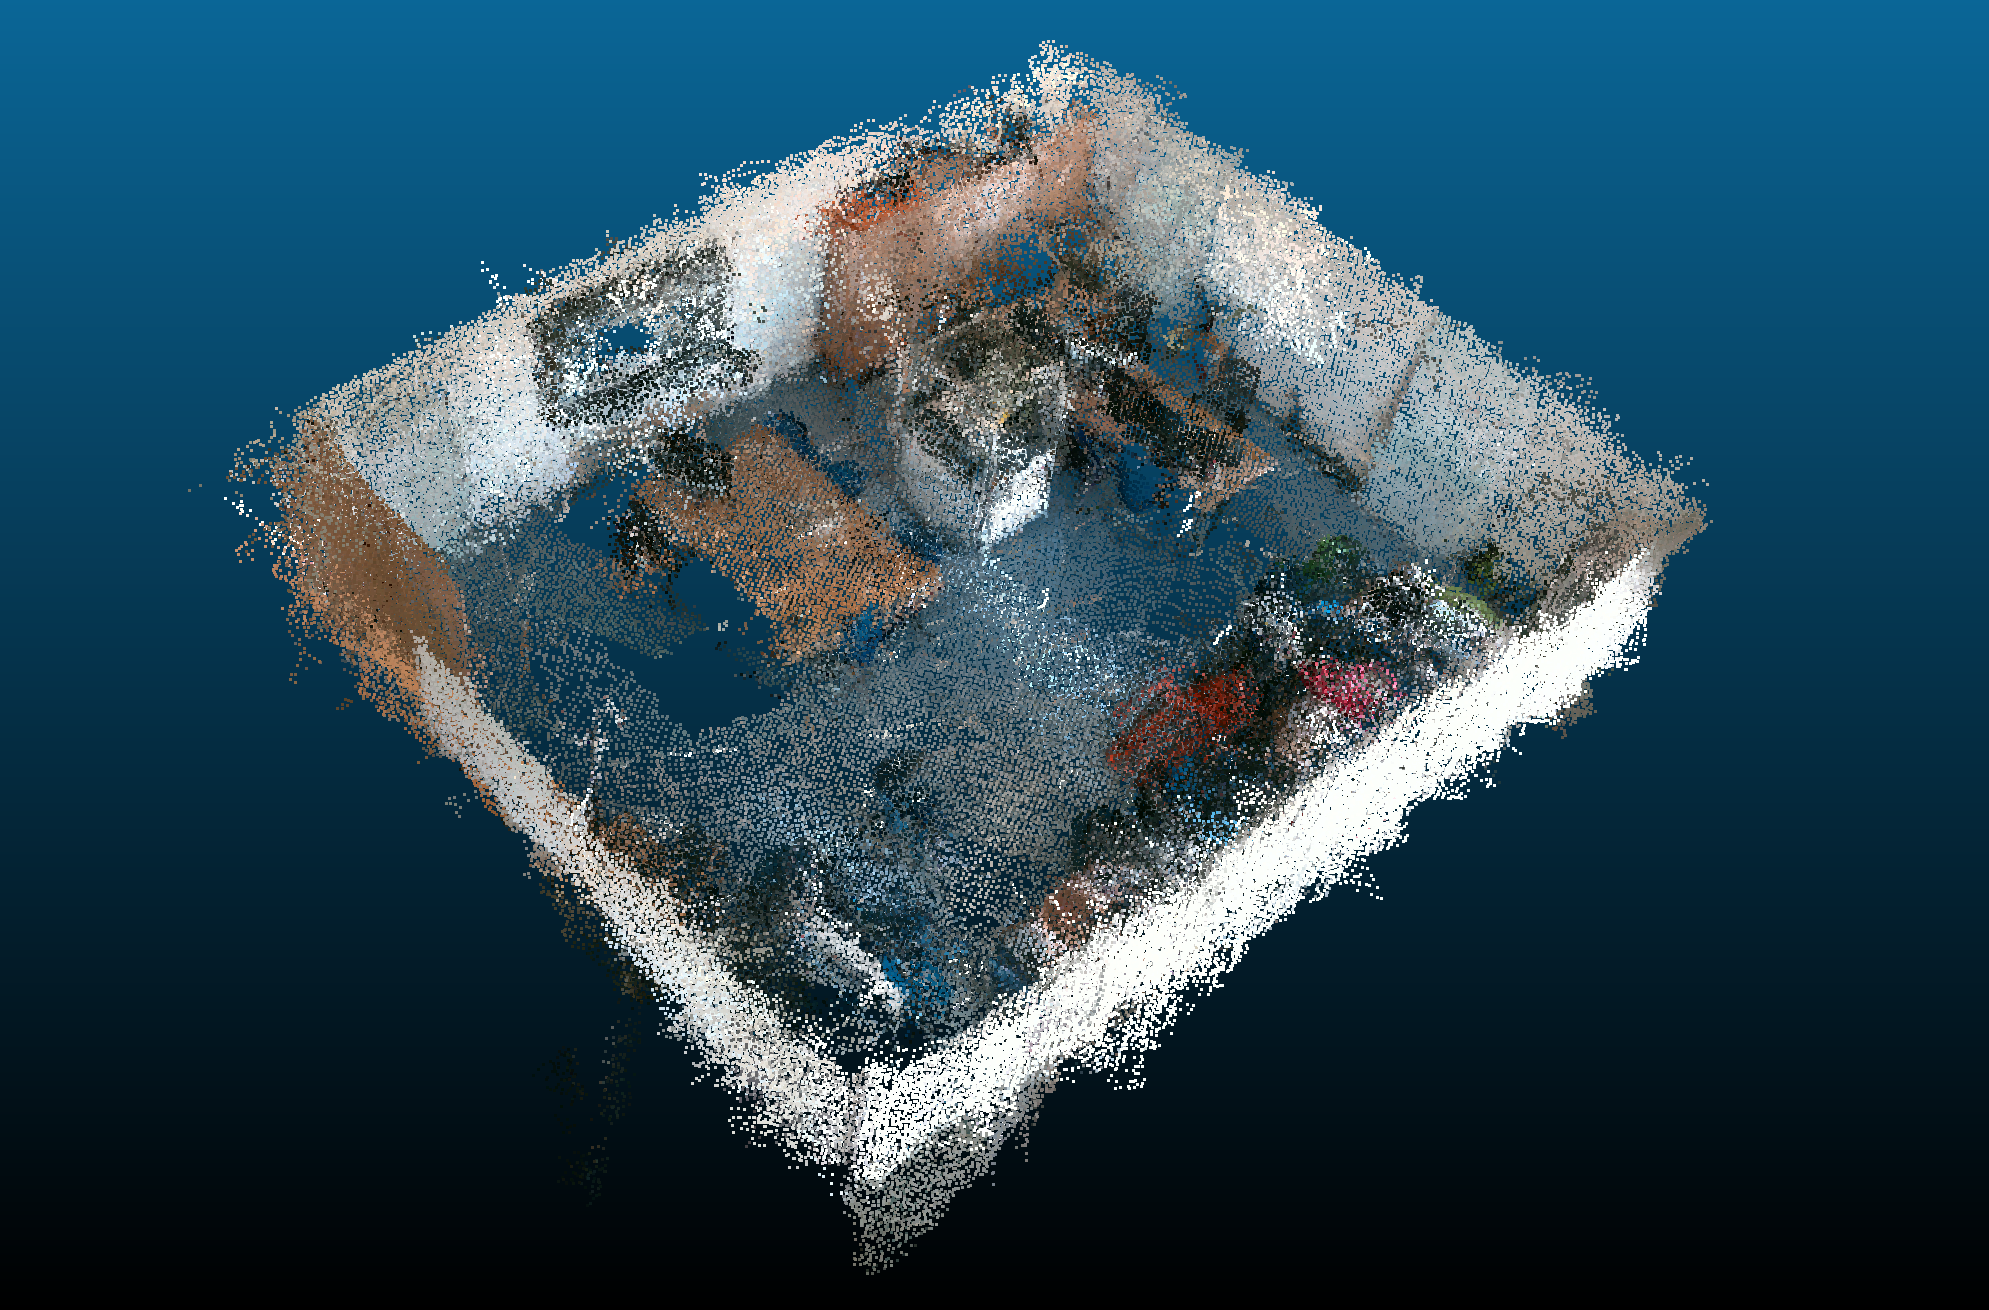
\includegraphics[width=0.9\linewidth]{images/425.png}
        \caption[Dynamic Dataset office]{}
        \label{fig:fin425}
    \end{subfigure}
    \begin{subfigure}{0.5\textwidth}
        \centering
        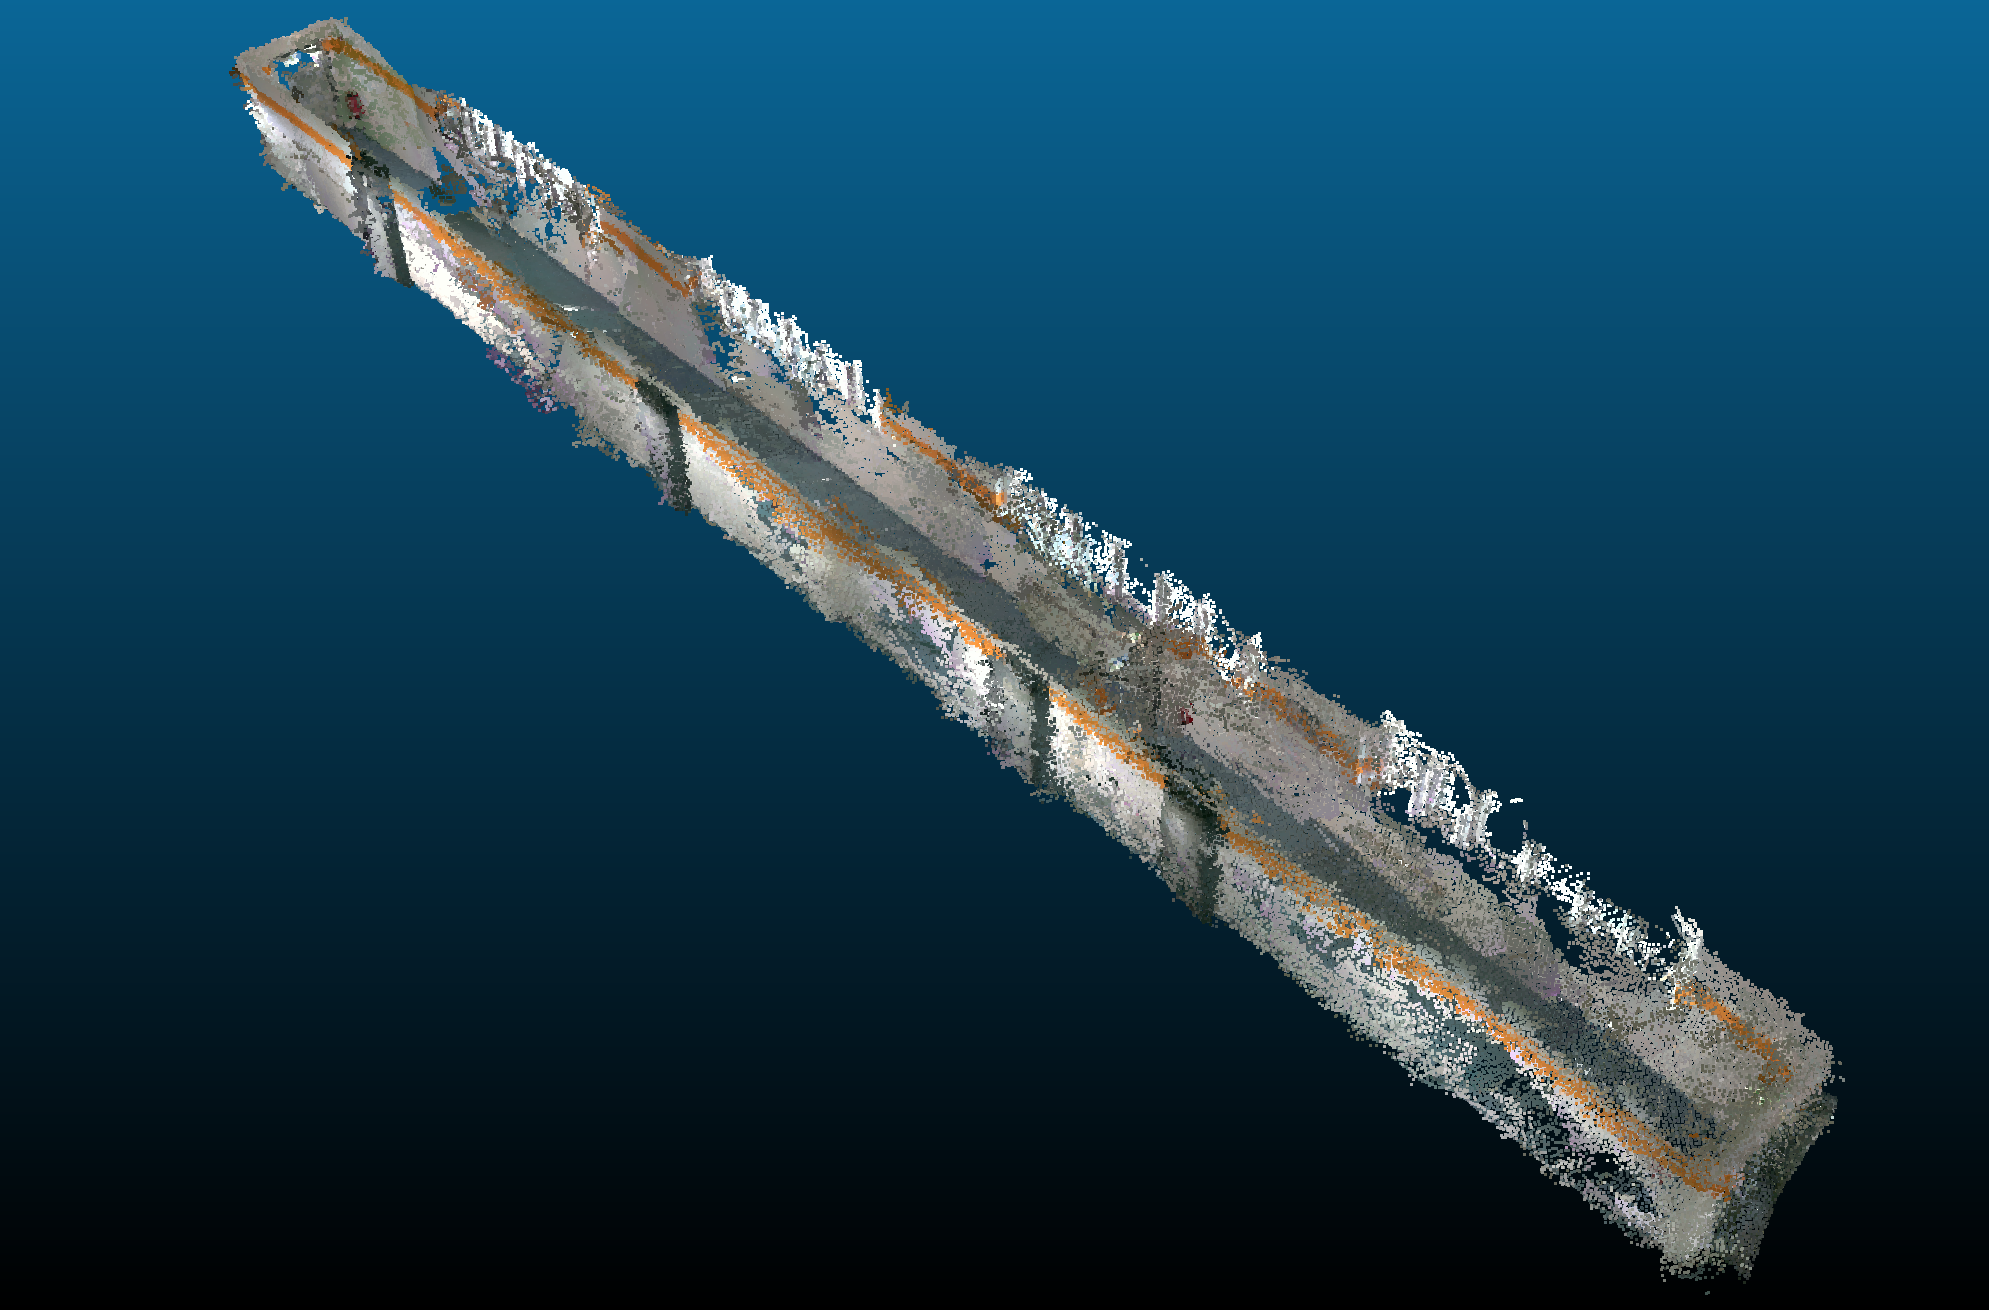
\includegraphics[width=0.9\linewidth]{images/hallway.png}
        \caption[Dynamic Dataset office]{}
        \label{fig:finhw}
    \end{subfigure}
    \caption[Dynamic Datasets]{The recorded point clouds for each scene type: (a) auditorium, (b) conference room, (c) office and (d) hallway.
        The ceilings have been manually removed for visualization purposes but remain in the dataset for the experiments.}
    \label{fig:fin}
\end{figure}


\section{Definition Real-Time}\label{sec:realtime}
Finally, as mentioned in Section~\ref{chap:Concept}, to determine whether or not an algorithm runs in real-time, we must first define the meaning of real-time.


In Subsection~\ref{subsec:pdaselect}, we introduce the differentiation between pre-processing and post-processing steps.
It is possible that one phase of an algorithm accounts for the majority of the total calculation time and that the algorithm
would be considered \textit{real-time} applicable, if that phase were to be excluded.
Because some steps can be covered by previous steps in the AR/VR system (see Figure~\ref{fig:concept}), i.e., by the sensor or the SLAM algorithm,
we give two definitions of \textit{real-time}.

In general, and without taking the algorithms internal structure into consideration, we have to consider possible
hardware limitations, data flow, and how often it is needed to perform calculations, e.g., how quickly the SLAM algorithm
updates the map (Figure~\ref{fig:concept}, [2]) or how frequent new planes are needed (Figure~\ref{fig:concept}, [4]).

The recorded raw data is not directly sent to the plane detection algorithm but instead given to RTAB-MAP, which then performs
calculations to update and publish the map.
Therefore, the upper limit is the frequency of how often RTAB-MAP publishes those updates, which by default is once per second.

\paragraph{Total Real-Time $RT_{tot}$}
According to this upper limit of RTAB-MAP, we consider an algorithm \textit{totally Real-Time} applicable, if it achieves an average frame
rate of minimum 1, e.g., the total processing time of an algorithm lies under one second. In the remainder of this work, we
use \textit{total Real-Time} and $RT_{tot}$ interchangeably.

\paragraph{Real-Time Plane Calculation $RT_{calc}$}
Being a subset of \textit{totally Real-Time applicability, Real-Time Plane Calculation} determines the real-time applicability if the processing time of an algorithm
\textit{excluding} pre-processing lies under the aforementioned upper bound of $1s$. Like $RT_{tot}$, we use
\textit{Real-Time Plane Calculation} and $RT_{calc}$ interchangeably.

%TODO  Eig nur needed wenn die algos langsamer sind als 1s ODER sollte die cloud extrem wachsen kann man sich auf die 6 meter beschränken, erstmal aber nicht}\\
% \subsection*{reduktion (opt)}
% We can reduce complexity further by taking the specifications (background)
% of the D455 into account. The RMS error of the D455 is reported to be 2\% at 4 meters distance to the sensor.
% Furthermore, the ideal distance is stated to range between $0.6 - 6$ meters.
% To maintain a dense and precise representation of our environment, we therefore limit the detection of planes to a
% radius of 6 meters from the current position.

\section{Summary}
Many applications have constraints in the form of a temporal component. Augmented or Virtual Reality applications that include plane detection
are no exception. In addition to time constraints, good quality is usually tightly coupled to expensive sensors.
In this work, we aim to evaluate the quality of real-time plane detection algorithms under the use of more affordable hardware, i.e., Intel RealSense.
At the beginning of this chapter, we state that three aspects are required for this evaluation, namely plane detection algorithms, a dataset, and a definition
of real-time.
The selection of the best plane detection algorithm, however, is non-trivial. After defining meaningful criteria for objective judgement, we
select appropriate plane detection algorithms. Moreover, we select two datasets, one of which is a novel creation,
and present two definitions of \textit{real-time} namely $RT_{tot}$ and $RT_{calc}$.
In Chapter~\ref{chap:eval}, we perform the evaluation.
\end{document}